% Options for packages loaded elsewhere
\PassOptionsToPackage{unicode}{hyperref}
\PassOptionsToPackage{hyphens}{url}
%
\documentclass[
]{article}
\usepackage{amsmath,amssymb}
\usepackage{iftex}
\ifPDFTeX
  \usepackage[T1]{fontenc}
  \usepackage[utf8]{inputenc}
  \usepackage{textcomp} % provide euro and other symbols
\else % if luatex or xetex
  \usepackage{unicode-math} % this also loads fontspec
  \defaultfontfeatures{Scale=MatchLowercase}
  \defaultfontfeatures[\rmfamily]{Ligatures=TeX,Scale=1}
\fi
\usepackage{lmodern}
\ifPDFTeX\else
  % xetex/luatex font selection
\fi
% Use upquote if available, for straight quotes in verbatim environments
\IfFileExists{upquote.sty}{\usepackage{upquote}}{}
\IfFileExists{microtype.sty}{% use microtype if available
  \usepackage[]{microtype}
  \UseMicrotypeSet[protrusion]{basicmath} % disable protrusion for tt fonts
}{}
\makeatletter
\@ifundefined{KOMAClassName}{% if non-KOMA class
  \IfFileExists{parskip.sty}{%
    \usepackage{parskip}
  }{% else
    \setlength{\parindent}{0pt}
    \setlength{\parskip}{6pt plus 2pt minus 1pt}}
}{% if KOMA class
  \KOMAoptions{parskip=half}}
\makeatother
\usepackage{xcolor}
\usepackage[margin=1in]{geometry}
\usepackage{color}
\usepackage{fancyvrb}
\newcommand{\VerbBar}{|}
\newcommand{\VERB}{\Verb[commandchars=\\\{\}]}
\DefineVerbatimEnvironment{Highlighting}{Verbatim}{commandchars=\\\{\}}
% Add ',fontsize=\small' for more characters per line
\usepackage{framed}
\definecolor{shadecolor}{RGB}{248,248,248}
\newenvironment{Shaded}{\begin{snugshade}}{\end{snugshade}}
\newcommand{\AlertTok}[1]{\textcolor[rgb]{0.94,0.16,0.16}{#1}}
\newcommand{\AnnotationTok}[1]{\textcolor[rgb]{0.56,0.35,0.01}{\textbf{\textit{#1}}}}
\newcommand{\AttributeTok}[1]{\textcolor[rgb]{0.13,0.29,0.53}{#1}}
\newcommand{\BaseNTok}[1]{\textcolor[rgb]{0.00,0.00,0.81}{#1}}
\newcommand{\BuiltInTok}[1]{#1}
\newcommand{\CharTok}[1]{\textcolor[rgb]{0.31,0.60,0.02}{#1}}
\newcommand{\CommentTok}[1]{\textcolor[rgb]{0.56,0.35,0.01}{\textit{#1}}}
\newcommand{\CommentVarTok}[1]{\textcolor[rgb]{0.56,0.35,0.01}{\textbf{\textit{#1}}}}
\newcommand{\ConstantTok}[1]{\textcolor[rgb]{0.56,0.35,0.01}{#1}}
\newcommand{\ControlFlowTok}[1]{\textcolor[rgb]{0.13,0.29,0.53}{\textbf{#1}}}
\newcommand{\DataTypeTok}[1]{\textcolor[rgb]{0.13,0.29,0.53}{#1}}
\newcommand{\DecValTok}[1]{\textcolor[rgb]{0.00,0.00,0.81}{#1}}
\newcommand{\DocumentationTok}[1]{\textcolor[rgb]{0.56,0.35,0.01}{\textbf{\textit{#1}}}}
\newcommand{\ErrorTok}[1]{\textcolor[rgb]{0.64,0.00,0.00}{\textbf{#1}}}
\newcommand{\ExtensionTok}[1]{#1}
\newcommand{\FloatTok}[1]{\textcolor[rgb]{0.00,0.00,0.81}{#1}}
\newcommand{\FunctionTok}[1]{\textcolor[rgb]{0.13,0.29,0.53}{\textbf{#1}}}
\newcommand{\ImportTok}[1]{#1}
\newcommand{\InformationTok}[1]{\textcolor[rgb]{0.56,0.35,0.01}{\textbf{\textit{#1}}}}
\newcommand{\KeywordTok}[1]{\textcolor[rgb]{0.13,0.29,0.53}{\textbf{#1}}}
\newcommand{\NormalTok}[1]{#1}
\newcommand{\OperatorTok}[1]{\textcolor[rgb]{0.81,0.36,0.00}{\textbf{#1}}}
\newcommand{\OtherTok}[1]{\textcolor[rgb]{0.56,0.35,0.01}{#1}}
\newcommand{\PreprocessorTok}[1]{\textcolor[rgb]{0.56,0.35,0.01}{\textit{#1}}}
\newcommand{\RegionMarkerTok}[1]{#1}
\newcommand{\SpecialCharTok}[1]{\textcolor[rgb]{0.81,0.36,0.00}{\textbf{#1}}}
\newcommand{\SpecialStringTok}[1]{\textcolor[rgb]{0.31,0.60,0.02}{#1}}
\newcommand{\StringTok}[1]{\textcolor[rgb]{0.31,0.60,0.02}{#1}}
\newcommand{\VariableTok}[1]{\textcolor[rgb]{0.00,0.00,0.00}{#1}}
\newcommand{\VerbatimStringTok}[1]{\textcolor[rgb]{0.31,0.60,0.02}{#1}}
\newcommand{\WarningTok}[1]{\textcolor[rgb]{0.56,0.35,0.01}{\textbf{\textit{#1}}}}
\usepackage{graphicx}
\makeatletter
\newsavebox\pandoc@box
\newcommand*\pandocbounded[1]{% scales image to fit in text height/width
  \sbox\pandoc@box{#1}%
  \Gscale@div\@tempa{\textheight}{\dimexpr\ht\pandoc@box+\dp\pandoc@box\relax}%
  \Gscale@div\@tempb{\linewidth}{\wd\pandoc@box}%
  \ifdim\@tempb\p@<\@tempa\p@\let\@tempa\@tempb\fi% select the smaller of both
  \ifdim\@tempa\p@<\p@\scalebox{\@tempa}{\usebox\pandoc@box}%
  \else\usebox{\pandoc@box}%
  \fi%
}
% Set default figure placement to htbp
\def\fps@figure{htbp}
\makeatother
\setlength{\emergencystretch}{3em} % prevent overfull lines
\providecommand{\tightlist}{%
  \setlength{\itemsep}{0pt}\setlength{\parskip}{0pt}}
\setcounter{secnumdepth}{-\maxdimen} % remove section numbering
\usepackage{bookmark}
\IfFileExists{xurl.sty}{\usepackage{xurl}}{} % add URL line breaks if available
\urlstyle{same}
\hypersetup{
  pdftitle={Labs using R:  10. ANOVA},
  hidelinks,
  pdfcreator={LaTeX via pandoc}}

\title{Labs using R: 10. ANOVA}
\author{}
\date{\vspace{-2.5em}}

\begin{document}
\maketitle

{
\setcounter{tocdepth}{3}
\tableofcontents
}
\emph{This lab is part of a series designed to accompany a course using
}The Analysis of Biological Data\emph{. The rest of the labs can be
found \href{index.html}{here}. This lab is based on topics in Chapter 15
of ABD.}

\section{Learning outcomes}\label{learning-outcomes}

\begin{itemize}
\item
  Use R to perform analysis of variance (ANOVA) to compare the means of
  multiple groups.
\item
  Perform Tukey-Kramer tests to look at unplanned contrasts between all
  pairs of groups.
\item
  Use Kruskal-Wallis tests to test for difference between groups without
  assumptions of normality.
\end{itemize}

If you have not already done so, download \href{ABDLabs.zip}{the zip
file containing Data, R scripts, and other resources for these labs}.
Remember to start RStudio from the ``ABDLabs.Rproj'' file in that folder
to make these exercises work more seamlessly.

\begin{center}\rule{0.5\linewidth}{0.5pt}\end{center}

\section{Learning the tools}\label{learning-the-tools}

For the examples in this lab, we will again return to the Titanic data
set. We'll group passengers by the passenger class they travelled under
(a categorical variable) and ask whether different passenger classes
differed in their mean age (a numerical variable).

First, load the data.

\begin{Shaded}
\begin{Highlighting}[]
\NormalTok{titanicData }\OtherTok{\textless{}{-}} \FunctionTok{read.csv}\NormalTok{(}\StringTok{"DataForLabs/titanic.csv"}\NormalTok{, }\AttributeTok{stringsAsFactors =} \ConstantTok{TRUE}\NormalTok{)}
\end{Highlighting}
\end{Shaded}

Let's first look at the data to get a sense of how well it fits the
assumptions of ANOVA. Multiple histogram are useful for this purpose. As
we saw in the last lab, we can use \textbf{ggplot()} and facets to make
this plot:

\begin{Shaded}
\begin{Highlighting}[]
\FunctionTok{library}\NormalTok{(ggplot2)}

\FunctionTok{ggplot}\NormalTok{(titanicData, }\FunctionTok{aes}\NormalTok{(}\AttributeTok{x =}\NormalTok{ age)) }\SpecialCharTok{+}   
  \FunctionTok{geom\_histogram}\NormalTok{() }\SpecialCharTok{+} 
  \FunctionTok{facet\_wrap}\NormalTok{(}\SpecialCharTok{\textasciitilde{}}\NormalTok{ passenger\_class, }\AttributeTok{ncol =} \DecValTok{1}\NormalTok{) }
\end{Highlighting}
\end{Shaded}

\begin{verbatim}
## `stat_bin()` using `bins = 30`. Pick better value with `binwidth`.
\end{verbatim}

\begin{verbatim}
## Warning: Removed 680 rows containing non-finite outside the scale range (`stat_bin()`).
\end{verbatim}

\pandocbounded{
\includegraphics[keepaspectratio]{R_tutorial_ANOVA_files/figure-latex/unnamed-chunk-2-1.pdf}}

These data look sufficiently normal and with similar spreads that ANOVA
would be appropriate.

To confirm these visual impressions, it would be useful to construct a
table of the means and standard deviations of each group. There are
numerous ways to do this in R, but one of the neatest is to use
functions from the package \textbf{dplyr}. If you have not done so yet,
install the \textbf{dplyr} package from the ``Packages'' tab in RStudio.
Then load the \textbf{dplyr} package with \textbf{library()}.

\begin{Shaded}
\begin{Highlighting}[]
\FunctionTok{library}\NormalTok{(dplyr)}
\end{Highlighting}
\end{Shaded}

\subsubsection{group\_by()}\label{group_by}

The package \textbf{dplyr} has several useful features for manipulating
data sets. For our current purposes, we will find two functions
particularly useful: \textbf{group\_by()} and \textbf{summarise()}.
These two functions are well named and work together well, first to
organize the data by groups, and second to summarize the results for
each group.

First, use \textbf{group\_by()} to organize your data frame by the
appropriate grouping variable. For example, here we want to organize the
\textbf{titanicData} by \textbf{passenger\_class}:

\begin{Shaded}
\begin{Highlighting}[]
\NormalTok{titanic\_by\_passenger\_class }\OtherTok{\textless{}{-}} \FunctionTok{group\_by}\NormalTok{(titanicData,passenger\_class)}
\end{Highlighting}
\end{Shaded}

\subsubsection{summarise()}\label{summarise}

After applying \textbf{group\_by()} to a data frame, we can summarize
the data using \textbf{summarise()}. (The ``s'' in \textbf{summarise()}
is not a typo---the creator of the package is from New Zealand.) With
\textbf{summarise()}, we can apply any type of function that summarizes
data (e.g.~\textbf{mean()}, \textbf{median()}, \textbf{var()}, etc.),
and receive that summary group by group. For example, to calculate the
mean age of each \textbf{passenger\_class}, we can use:

\begin{Shaded}
\begin{Highlighting}[]
\FunctionTok{summarise}\NormalTok{(titanic\_by\_passenger\_class, }\AttributeTok{group\_mean =} \FunctionTok{mean}\NormalTok{(age, }\AttributeTok{na.rm=}\ConstantTok{TRUE}\NormalTok{))}
\end{Highlighting}
\end{Shaded}

\begin{verbatim}
## # A tibble: 3 x 2
##   passenger_class group_mean
##   <fct>                <dbl>
## 1 1st                   39.7
## 2 2nd                   28.3
## 3 3rd                   24.5
\end{verbatim}

As input, we give the name of the grouped table created by
\textbf{group\_by()} and the function we want to apply to each group. In
this case we used \textbf{mean(age, na.rm=TRUE)}.
``\textbf{group\_mean}'' is a name we give to that summary variable (it
could have been any name we wanted). The output looks like a table and
includes the names of the groups being summarized. (A ``tibble'' is not
how New Zealanders spell ``table'', but is a type of table like a data
frame.) ``3 x 2'' here refers to the number of rows x columns in the
``tibble'' output.

We can give \textbf{summarise()} many summary functions at once, and it
will create columns in the output table for each one. For example, if we
want to output both the mean and the standard deviation, we can add
\textbf{sd = sd(age, na.rm=TRUE)} to the function above.

\begin{Shaded}
\begin{Highlighting}[]
\FunctionTok{summarise}\NormalTok{(titanic\_by\_passenger\_class, }\AttributeTok{group\_mean =} \FunctionTok{mean}\NormalTok{(age, }\AttributeTok{na.rm=}\ConstantTok{TRUE}\NormalTok{), }\AttributeTok{group\_sd =} \FunctionTok{sd}\NormalTok{(age, }\AttributeTok{na.rm=}\ConstantTok{TRUE}\NormalTok{))}
\end{Highlighting}
\end{Shaded}

\begin{verbatim}
## # A tibble: 3 x 3
##   passenger_class group_mean group_sd
##   <fct>                <dbl>    <dbl>
## 1 1st                   39.7     14.9
## 2 2nd                   28.3     13.0
## 3 3rd                   24.5     11.3
\end{verbatim}

Note that the standard deviations are very similar, which means that
these data fit the equal variance assumption of ANOVA.

\subsection{ANOVA}\label{anova}

Analysis of variance (or ANOVA) is not quite as simple in R as one might
hope. Doing ANOVA takes at least two steps. First, we fit the ANOVA
model to the data using the function \textbf{lm()}. This step carries
out a bunch of intermediate calculations. Second, we use the results of
first step to do the ANOVA calculations and place them in an ANOVA table
using the function \textbf{anova()}. The function name \textbf{lm()}
stands for ``linear model''; this is actually a very powerful function
that allows a variety of calculations. One-way ANOVA is a type of linear
model.

\subsubsection{lm()}\label{lm}

The function \textbf{lm()} needs a formula and a data frame as
arguments. The formula is a statement specifying the ``model'' that we
are asking R to fit to the data. A model formula always takes the form
of a response variable, followed by a tilde(\textbf{\textasciitilde{}}),
and then at least one explanatory variable. In the case of a one-way
ANOVA, this model statement will take the form

\begin{Shaded}
\begin{Highlighting}[]
\NormalTok{numerical\_variable }\SpecialCharTok{\textasciitilde{}}\NormalTok{ categorical\_variable}
\end{Highlighting}
\end{Shaded}

For example, to compare differences in mean age among passenger classes
on the Titanic, this formula is

\begin{Shaded}
\begin{Highlighting}[]
\NormalTok{age }\SpecialCharTok{\textasciitilde{}}\NormalTok{ passenger\_class}
\end{Highlighting}
\end{Shaded}

This formula tells R to ``fit'' a model in which the ages of passengers
are grouped by the variable \textbf{passenger\_class}.

The name of the data frame containing the variables stated in the
formula is the second argument of \textbf{lm()}. Finally, to complete
the \textbf{lm()} command, it is necessary to save the intermediate
results by assigning them to a new object, which \textbf{anova()} can
then use to make the ANOVA table. For example, here we assign the
results of \textbf{lm()} to a new object named
``\textbf{titanicANOVA}'':

\begin{Shaded}
\begin{Highlighting}[]
\NormalTok{titanicANOVA }\OtherTok{\textless{}{-}} \FunctionTok{lm}\NormalTok{(age }\SpecialCharTok{\textasciitilde{}}\NormalTok{ passenger\_class, }\AttributeTok{data =}\NormalTok{ titanicData)}
\end{Highlighting}
\end{Shaded}

\subsubsection{anova()}\label{anova-1}

The function \textbf{anova()} takes the results of \textbf{lm()} as
input and returns an ANOVA table as output:

\begin{Shaded}
\begin{Highlighting}[]
\FunctionTok{anova}\NormalTok{(titanicANOVA)}
\end{Highlighting}
\end{Shaded}

\begin{verbatim}
## Analysis of Variance Table
## 
## Response: age
##                  Df Sum Sq Mean Sq F value    Pr(>F)    
## passenger_class   2  26690 13344.8  75.903 < 2.2e-16 ***
## Residuals       630 110764   175.8                      
## ---
## Signif. codes:  0 '***' 0.001 '**' 0.01 '*' 0.05 '.' 0.1 ' ' 1
\end{verbatim}

This table shows the results of a test of the null hypothesis that the
mean ages are the same among the three groups. The \emph{P}-value is
very small, and so we reject the null hypothesis of no differences in
mean age among the passenger classes.

\subsection{Tukey-Kramer test}\label{tukey-kramer-test}

A single-factor ANOVA can tell us that at least one group has a
different mean from another group, but it does not inform us which group
means are different from which other group means. A Tukey-Kramer test
lets us test the null hypothesis of no difference between the population
means for all pairs of groups. The Tukey-Kramer test (also known as a
Tukey Honest Significance Test, or Tukey HSD), is implemented in R in
the function \textbf{TukeyHSD()}.

We will use the results of an ANOVA done with \textbf{lm()} as above,
that we stored in the variable \textbf{titanicANOVA}. To do a
Tukey-Kramer test on these data, we need to first apply the function
\textbf{aov()} to \textbf{titanicANOVA}, and then we need to apply the
function \textbf{TukeyHSD} to the result. We can do this in a single
command:

\begin{Shaded}
\begin{Highlighting}[]
\FunctionTok{TukeyHSD}\NormalTok{(}\FunctionTok{aov}\NormalTok{(titanicANOVA))}
\end{Highlighting}
\end{Shaded}

\begin{verbatim}
##   Tukey multiple comparisons of means
##     95% family-wise confidence level
## 
## Fit: aov(formula = titanicANOVA)
## 
## $passenger_class
##               diff        lwr        upr     p adj
## 2nd-1st -11.367459 -14.345803  -8.389115 0.0000000
## 3rd-1st -15.148115 -18.192710 -12.103521 0.0000000
## 3rd-2nd  -3.780656  -6.871463  -0.689849 0.0116695
\end{verbatim}

The key part of this output is the table at the bottom. It estimates the
difference between the means of groups (for example, the 2nd passenger
class compared to the 1st passenger class) and calculates a 95\%
confidence interval for the difference between the corresponding
population means. (``\textbf{lwr}'' and ``\textbf{upr}'' correspond to
the lower and upper bounds of that confidence interval for the
difference in means.) Finally, it give the \emph{P}-value from a test of
the null hypothesis of no difference between the means (the column
headed with ``\textbf{p adj}''). In the case of the Titanic data,
\emph{P} is less than 0.05 in all pairs, and we therefore reject every
null hypothesis. We conclude that the population mean ages of all
passenger classes are significantly different from each other.

\subsection{Kruskal-Wallis test}\label{kruskal-wallis-test}

A Kruskal-Wallis test is a non-parametric analog of a one-way ANOVA. It
does not assume that the variable has a normal distribution. (Instead,
it tests whether the variable has the same distribution with the same
mean in each group.)

To run a Kruskal-Wallis test, use the R function
\textbf{kruskal.test()}. The input for this function is the same as we
used for \textbf{lm()} above. It includes a model formula statement and
the name of the data frame to be used.

\begin{Shaded}
\begin{Highlighting}[]
\FunctionTok{kruskal.test}\NormalTok{(age }\SpecialCharTok{\textasciitilde{}}\NormalTok{ passenger\_class, }\AttributeTok{data =}\NormalTok{ titanicData)}
\end{Highlighting}
\end{Shaded}

\begin{verbatim}
## 
##  Kruskal-Wallis rank sum test
## 
## data:  age by passenger_class
## Kruskal-Wallis chi-squared = 116.08, df = 2, p-value < 2.2e-16
\end{verbatim}

You can see for the output that a Kruskal-Wallis test also strongly
rejects the null hypothesis of equality of age for all passenger class
groups with the Titanic data.

\section{R commands summary}\label{r-commands-summary}

\pandocbounded{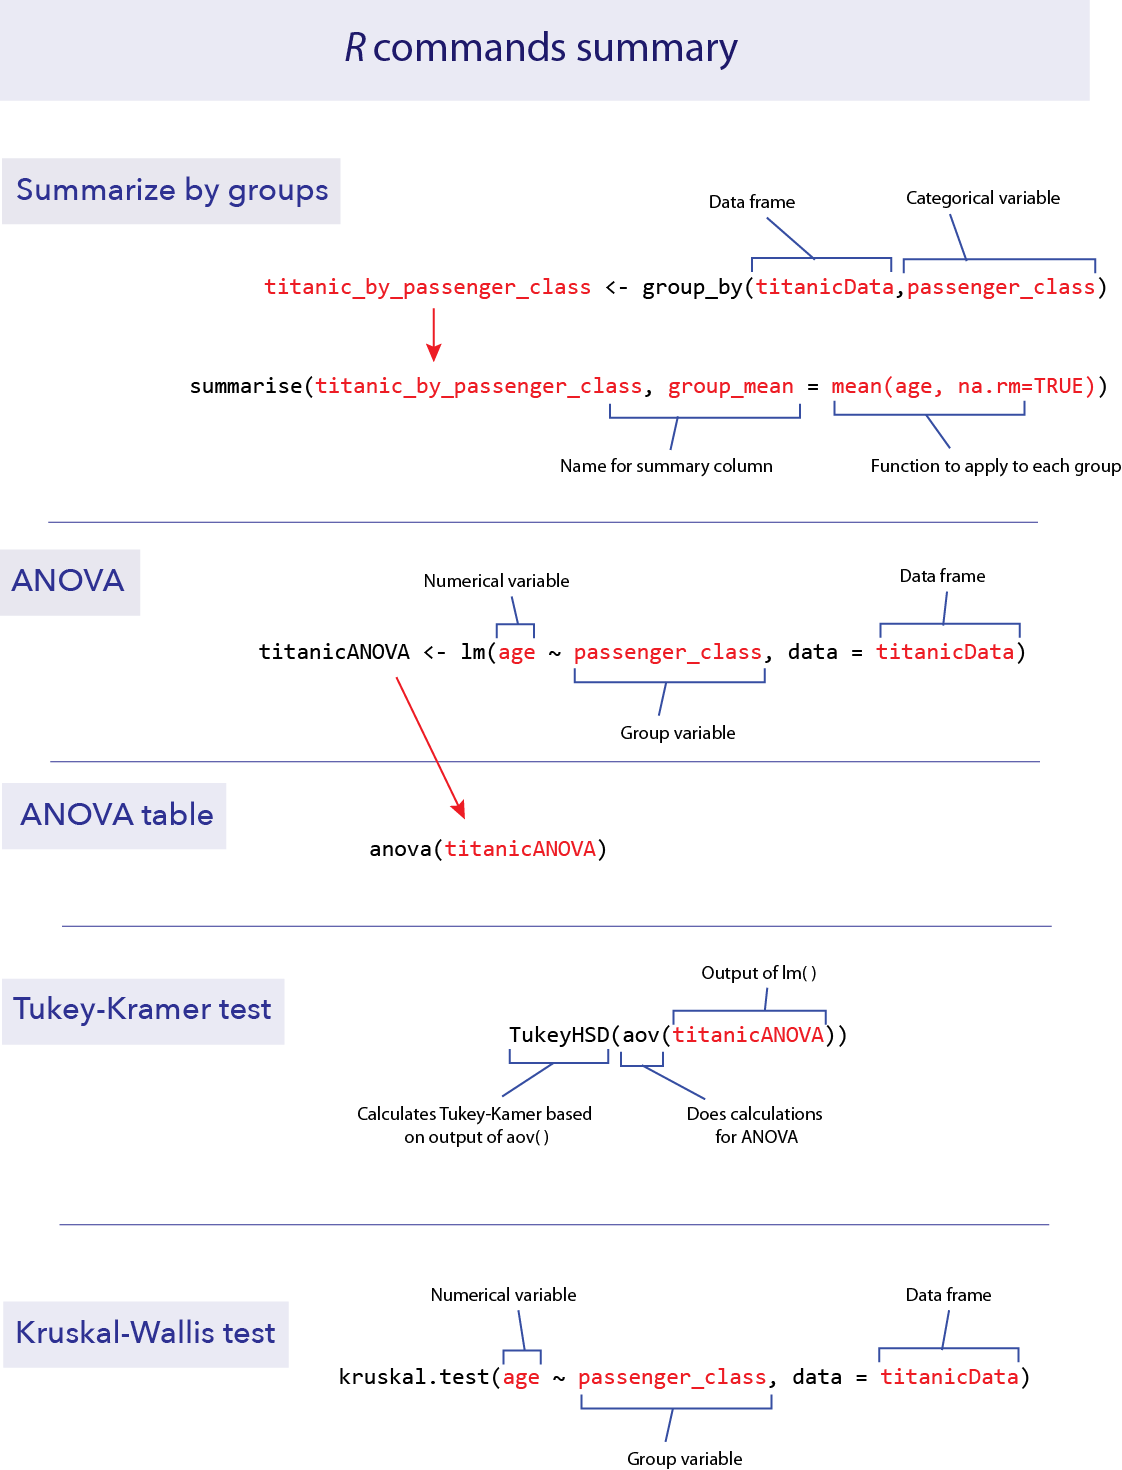
\includegraphics[keepaspectratio]{formula_summaries/ANOVA summary.png}}

\begin{center}\rule{0.5\linewidth}{0.5pt}\end{center}

\section{Questions}\label{questions}

1. The European cuckoo does not look after its own eggs, but instead
lays them in the nests of birds of other species. Previous studies
showed that cuckoos sometimes have evolved to lay eggs that are colored
similarly to the host bird species' eggs. Is the same true of egg size
-- do cuckoos lay eggs similar in size to the size of the eggs of their
hosts? The data file ``cuckooeggs.csv'' contains data on the lengths of
cuckoo eggs laid in the nests of a variety of host species. Here we
compare the mean size of cuckoo eggs found in the nests of different
host species.

\begin{enumerate}
\def\labelenumi{\alph{enumi}.}
\item
  Plot a multiple histogram showing cuckoo egg lengths by host species.
\item
  Calculate a table that shows the mean and standard deviation of length
  of cuckoo eggs for each host species.
\item
  Look at the graph and the table. For these data, would ANOVA be a
  valid method to test for differences between host species in the
  lengths of cuckoo eggs in their nests?
\item
  Use ANOVA to test for a difference between host species in the mean
  size of the cuckoo eggs in their nests. What is your conclusion?
\item
  Assuming that ANOVA rejected the null hypotheses of no mean
  differences, use a Tukey-Kramer test to decide which pairs of host
  species are significantly different from each other in cuckoo egg mean
  length. What is your conclusion?
\end{enumerate}

2. The pollen of the maize (corn) plant is a source of food to larval
mosquitoes of the species \emph{Anopheles arabiensis}, the main vector
of malaria in Ethiopia. The production of maize has increased
substantially in certain areas of Ethiopia recently, and over the same
time period, malaria has entered in to new areas where it was previously
rare. This raises the question, is the increase of maize cultivation
partly responsible for the increase in malaria?

One line of evidence is to look for an association between maize
production and malaria incidence at different geographically dispersed
sites (Kebede et al.~2005). The data set ``malaria vs maize.csv''
contains information on several high-altitude sites in Ethiopia, with
information about the level of cultivation of maize (low, medium or high
in the variable \textbf{maize\_yield}) and the rate of malaria per
10,000 people (\textbf{incidence\_rate\_per\_ten\_thousand}).

\begin{enumerate}
\def\labelenumi{\alph{enumi}.}
\item
  Plot a multiple histogram to show the relationship between level of
  maize production and the incidence of malaria.
\item
  ANOVA is a logical choice of method to test differences in the mean
  rate of malaria between sites differing in level of maize production.
  Calculate the standard deviation of the incidence rate for each level
  of maize yield. Do these data seem to conform to the assumptions of
  ANOVA? Describe any violations of assumptions you identify.
\item
  Compute the log of the incidence rate and redraw the multiple
  histograms for different levels of maize yield. Calculate the standard
  deviation of the log incidence rate for each level of maize yield.
  Does the log-transformed data better meet the assumptions of ANOVA
  than did the untransformed data?
\item
  Test for an association between maize yield and malaria incidence.
\end{enumerate}

3. Animals that are infected with a pathogen often have disturbed
circadian rhythms. (A circadian rhythm is an endogenous daily cycle in a
behavior or physiological trait that persists in the absence of time
cues.) Shirasu-Hiza et al.~(2007) wanted to know whether it was possible
that the circadian timing mechanism itself could have an effect on
disease. To test this idea they sampled from three groups of fruit
flies: one ``normal'', one with a mutation in the timing gene
\emph{tim01}, and one group that had the \emph{tim01} mutant in a
heterozygous state. They exposed these flies to a dangerous bacteria,
\emph{Streptococcus pneumoniae}, and measured how long the flies lived
afterwards, in days. The date file ``circadian mutant health.csv'' shows
some of their data.

\begin{enumerate}
\def\labelenumi{\alph{enumi}.}
\item
  Plot a histogram of each of the three groups. Do these data match the
  assumptions of an ANOVA?
\item
  Use a Kruskal-Wallis test to ask whether lifespan differs between the
  three groups of flies.
\end{enumerate}

\end{document}
